% This is samplepaper.tex, a sample chapter demonstrating the
% LLNCS macro package for Springer Computer Science proceedings;
% Version 2.20 of 2017/10/04
%
\documentclass[runningheads]{llncs}
%
\usepackage{graphicx}
% Used for displaying a sample figure. If possible, figure files should
% be included in EPS format.
%
% If you use the hyperref package, please uncomment the following line1
% to display URLs in blue roman font according to Springer's eBook style:
% \renewcommand\UrlFont{\color{blue}\rmfamily}

\begin{document}
%
\title{Gap Puzzles}

\subtitle{Puzzle solving using Prolog constraints}
%
%\titlerunning{Abbreviated paper title}
% If the paper title is too long for the running head, you can set
% an abbreviated paper title here
%
\author{João Pedro Pinheiro de Lacerda Campos\inst{1,2} \and
Leonardo Fernandes Moura\inst{1,2}}
%
\authorrunning{J. Campos L. Moura}
% First names are abbreviated in the running head.
% If there are more than two authors, 'et al.' is used.
%

\institute{
Faculdade de Engenharia da Universidade do Porto,
Rua Dr. Roberto Frias, s/n 4200-465 Porto PORTUGAL
\email{feup@fe.up.pt}\\
\url{http://www.fe.up.pt} \and
Logical Programing Course, Class 3MIEIC03, Group Gap Puzzle\_5}

%
\maketitle              % typeset the header of the contribution
%
\begin{abstract}
This project was developed during the the Logical Programing Course in the context of the year
of the Integrated Masters in Informatics and Computing Engineering at The Faculty of Engineering
of the University of Porto. The goal was to solve a problem using the Prolog programming language,
more specifically, using Constraint Logic Programming over Finite Domains (clpfd) library, that's defined
in the SICStus Prolog distribution.
In the specific case of our team, the problem in question is the Gap Puzzle, which is defined in detail in
\textbf{Section 2}.
In order to solve the problem, Prolog constraint programming was used. This type of programming grants us the
advantage of fast computation, requiring a somewhat simple and little verbosed kind of programming. Using constraints,
we can simply define all the constraints of our problem (in the case of puzzles these are the rules of the puzzle),
which in the case of more complex problems is not trivial. Then, after defining the solution search algorithm,
the clpfd library will search for solutions.


\keywords{Prolog  \and Constraint Programing \and Gap Puzzle.}
\end{abstract}

\pagebreak

\section{Introduction}
\paragraph{}
This goal of the project was to elaborate a Prolog program that, given a board order, computes all the solutions of the
Gap Puzzle for that board order.
Optimization is a relevant factor here. Different ways of defining constraints can lead us to the same set of
solutions, but computation times can vary greatly. So, one of the concerns during the development of this project
was to find solutions as fast as possible.

\paragraph{}
Bellow we shortly explain the following sections of this article.

\begin{itemize}
    \item \textbf{Problem Description:} Detailed description of the problem we are solving and the rules of Gap Puzzles

    \item \textbf{Approach:} Description of choices made through out the project
    \begin{itemize}
        \item \textbf{Decision Variables}
        \item \textbf{Constraints}
        \item \textbf{Search Strategy}
    \end{itemize}

    \item \textbf{Solution Presentation:} Description of how solutions are presented in an intelligible way.
    \item \textbf{Results:} Examples of tests with different search strategies
    \item \textbf{Conclusions:} Conclusions taken from the work and what could have been improved
\end{itemize}

\section{Problem Description}
The problem in question is the solution of the Gap Puzzle. Gap is a very simple puzzle, yet a challenging
one. We have grid of arbitrary size and our goal, is to shade two squares of the grid in every row and column, such that
two shaded squares do not touch, even at the corners. Because there is more than one solution for every grid order,
in the puzzle form of the problem, there are numbers on the side of the grid to indicate the number of non shaded squares
there must exist between two shaded squares in that row or column. The figure below illustrates an example of puzzle with
order 9.

\begin{figure}
    \begin{center}
        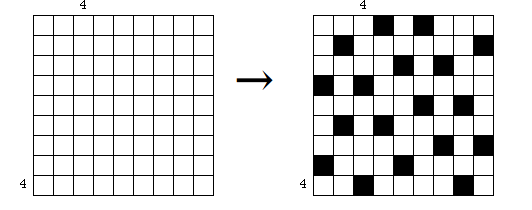
\includegraphics[scale=0.5]{images/figure1.png}
        \caption{Gap Puzzle example} \label{fig1}
    \end{center}
\end{figure}

\paragraph{}
Although they are very interesting, these specific puzzles do not interest us. We are interested in finding arbitrary
solutions for a problem with a given order.

\pagebreak

\section{Approach}
\paragraph{}
In the specific context of this problem, the constraints used to solve the problem are a translation of the rules of
the puzzle to Prolog Constraints. The following subsections explain the constraints used in detail.

\subsection{Decision Variables}
To solve this problem we have only a decision variable, the \textit{Points} list. This list stores the coordinates of all
the cells that will be shaded, in the format \textit{[X1,Y1,X2,Y2|...]}. We start by defining that this list will have a
a length of:

\begin{equation}
    points = 2 * order
\end{equation}
\begin{equation}
    length = 4 * order
\end{equation}

This happens because we can only have two shaded cells in each row. Since the number of rows is equal to the order of our
grid, we a number of points that is two times our order.

\paragraph{}
Then we define the domain of the decision variable, which is between zero and the number immediately inferior to our order,
this is because we are considering a system of coordinates starting in zero.

\subsection{Constraints}
\paragraph{}
The first constraint we make is to ensure there are only two shaded cells in each row and in each column. We do this
using the \textbf{restrict\_two(+List,+Order)} predicate. This predicate restricts each number of the domain in the list
to occur exactly two times in the list. We do this two times, the first for a list containing all the X coordinates of the
solution, and a second time for the Y coordinate. We are able to split this using the \textbf{extractX(+List,-XList)} and
\textbf{extractY(+List,-YList)} predicates. The first one takes a list with the solution format and unifies in
\textit{XList} all the X coordinates of that list. The \textit{extractY} predicate does the same for Y.

\begin{figure}
    \begin{center}
        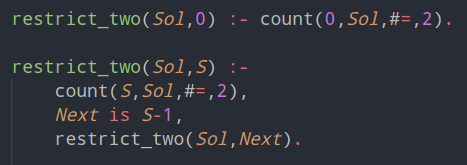
\includegraphics[scale=0.5]{images/restrict_two.png}
        \caption{The restrict\_two predicate} \label{fig2}
    \end{center}
\end{figure}

\paragraph{}
Then we restrict the positions of the shaded cells themselves. We do this using the \textbf{restrict\_next(+List)} predicate.
This predicate iterates through the list making sure that no other coordinates in the list are the coordinates of an
adjacent cell to the any of the other cells and that no two cell coordinates are the same. This predicate calls the
\textbf{restrict\_next\_pair(+List,+X,+Y)} predicate that applies the constraints mentioned above to all the other
coordinate pairs in the list.

\begin{figure}
    \begin{center}
        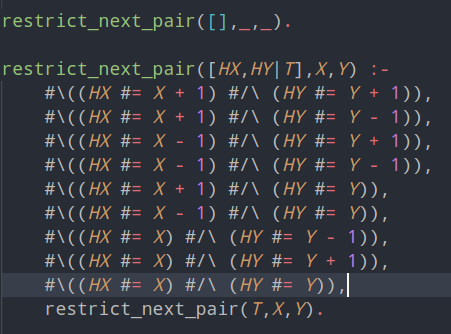
\includegraphics[scale=0.5]{images/restrictPair.png}
        \caption{The restrict\_next\_pair predicate} \label{fig3}
    \end{center}
\end{figure}

\subsection{Search Strategy}
\paragraph{}
For labeling we made an ordering function in \textbf{crescent\_order(+List)} predicate. This predicate orders the coordinates of the points
down-top and right-left, improving the labeling times for smaller boards.

\begin{figure}
    \begin{center}
        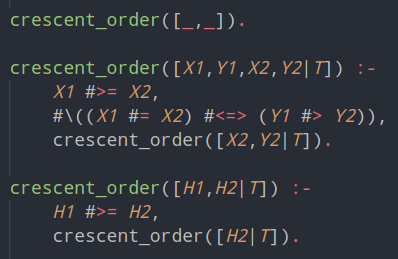
\includegraphics[scale=0.5]{images/crescent.png}
        \caption{Point ordering} \label{fig4}
    \end{center}
\end{figure}

\paragraph{}
For bigger boards, \textbf{crescent\_order(+List)} predicate is an expensive task, as it runs through the whole list of points to apply the restrictions.
For this reason, if the board is of order 15 or bigger, this predicate is not used.
\paragraph{}
We also added a random function that was given in the classes. This function allows \textbf{labeling} predicate to select the value in a random way.

\begin{figure}
    \begin{center}
        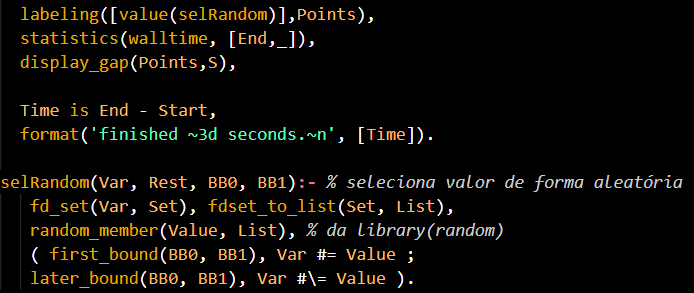
\includegraphics[scale=0.5]{images/random.png}
        \caption{Random selection predicate} \label{fig4}
    \end{center}
\end{figure}

\section{Solution Presentation}
\paragraph{}
For solution presentation we elaborated \textbf{display\_gap(+Sol,+Len)}. This predicate receives the \textit{Points}
list, with the format previously explained, and \textit{Order}, which is the order of the board the solution given applies to.
This predicate then uses the three predicates explained bellow.

\paragraph{}
Firstly it uses \textbf{empty\_board(-B,+Len)} predicate which creates a list of lists representing an empty grid, with order \textit{Len},
this new grid is then unified with \textit{B}.
This predicate works by appending new atoms, representing an empty cell (\textbf{' '},
a single space character) to an empty starting list. Once this list has the desired length, this list is then replicated
several times to form a new empty grid.

\paragraph{}
Then, we use the \textbf{process\_board(+Board,+Sol,-NewBoard)} to substitute all the empty cells in the positions given
by solution list, with the \textbf{' X '} atom.
This represents a shaded cell. In order to make the substitution we defined
the \textbf{replaceN(+List,+N,+NewElem,-Res)} predicate. This predicate substitutes the element of order \textit{N} in
\textit{List} to the element \textit{NewElem}, then unifies the resulting list with \textit{Res}.

\paragraph{}
Finally, the predicate \textbf{display\_board(+Board)} was defined to display the board \textit{Board}. This predicate
writes the separators in the screen and then displays each row of the grid, using the right format. Bellow, we can see a
displayed board.

\begin{figure}
    \begin{center}
        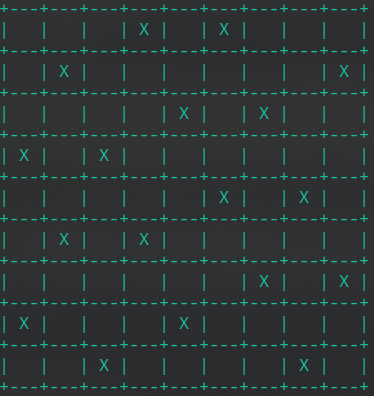
\includegraphics[scale=0.5]{images/fig2.png}
        \caption{Solution Display Example} \label{fig2}
    \end{center}
\end{figure}

\newpage

\section{Results}
\paragraph{}
Our program finds a solution given a valid number above 0. Given this, we tested it with all possible numbers from 1 to 30.
By doing this we discovered that the puzzle only has solutions for orders 9 and above. Here is one example of one board with order 11.

\begin{figure}
    \begin{center}
        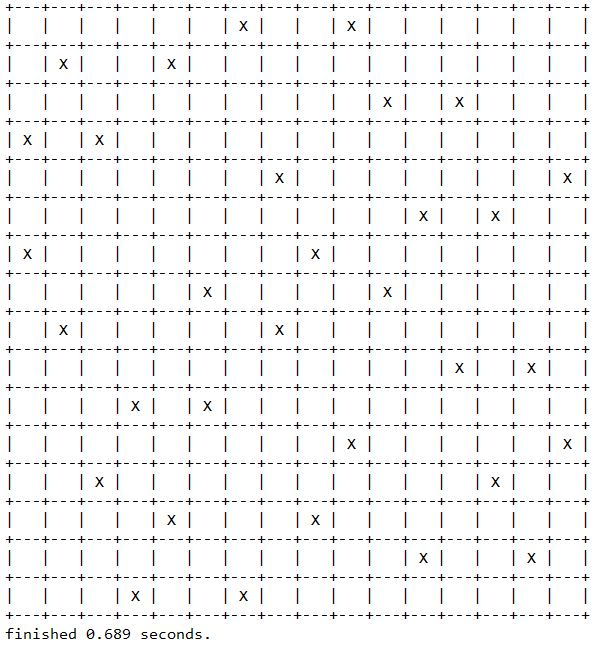
\includegraphics[scale=0.35]{images/gap9.jpg}
        \caption{Solution Example} \label{fig3}
    \end{center}
\end{figure}

\pagebreak

\paragraph{}
After making multiple tries per order we ended up with this graph. It shows the amount of time (in seconds) taken by the program for
each order. From the graph you can see a pattern where the program takes exponentially more time to solve the puzzle. But then it
reaches a point where there is a drop in that time. This pattern repeats itself after its first instance and probably forever, as you increase order.

\begin{figure}
    \begin{center}
        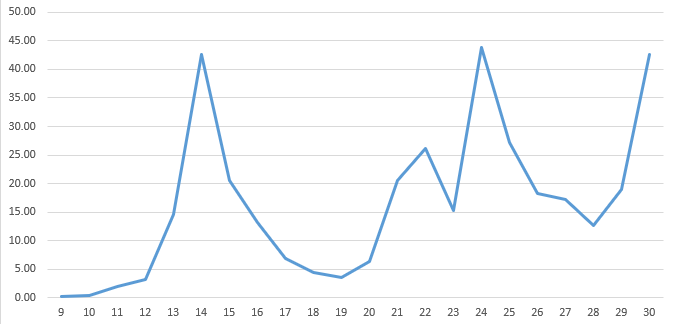
\includegraphics[scale=0.38]{images/graph.png}
        \caption{Times graph order/time(s)} \label{fig5}
    \end{center}
\end{figure}

\paragraph{}
This irregular behaviour told us the solution was imperfect somewhere. With that knowledge, we felt incentivized to search new ways of labeling variables.
Before we only ordered the values of the coordinates before labeling.
We then found we could add a random function to the labeling and once we implemented it, it showed incredible results.

\begin{figure}
    \begin{center}
        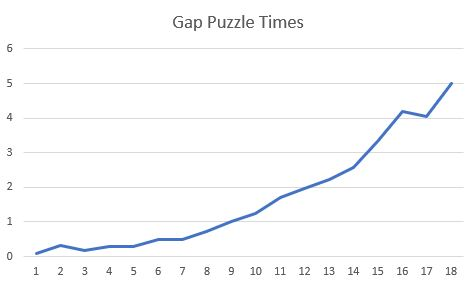
\includegraphics[scale=0.5]{images/graph2.png}
        \caption{Times graph after random labeling order/time(s)} \label{fig5}
    \end{center}
\end{figure}
After more testing, we reached the conclusion
that the best way to search for solutions in smaller boards was to use \textbf{crescent\_order(+List)}, but to bigger boards it wasted too much time. With this in mind,
we added a condition where if the board was of order 14 or below, it would use \textbf{crescent\_order(+List)}, but bigger boards it would not.
\begin{figure}
    \begin{center}
        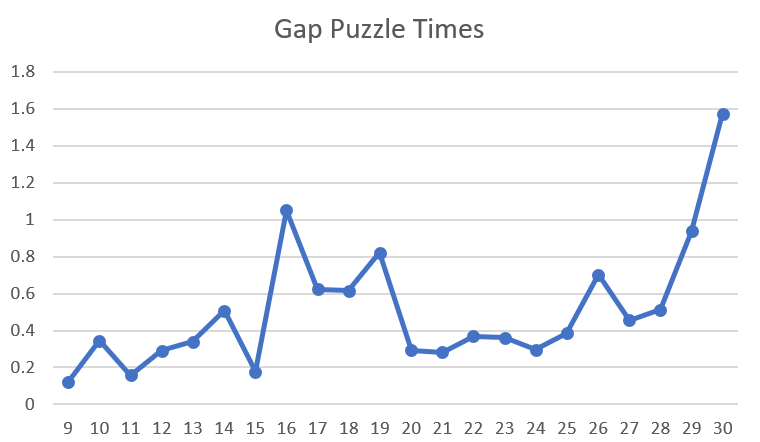
\includegraphics[scale=0.3]{images/graph3.png}
        \caption{Times graph after random labeling and condition for bigger boards \newline order/time(s)} \label{fig5}
    \end{center}
\end{figure}


\pagebreak
\section{Conclusions and Future Work}
\paragraph{}
We think we have achieved what was proposed to us at the start of this project. With this work we were able to learn how to think in a different way.
Since we use other paradigms of programming more frequently, when using prolog with restrictions we could not think of a solution to the problem as quickly as normal.
\paragraph{}
As previously said, the gap puzzle is a challenging one, but with the use of restrictions, we can find solutions in little time.
One significant thing we learned was that a change that might seem simple, as adding a random function, might increase efficiency by many times.
\paragraph{}
From the results we can conclude that our program is quite efficient and that is one of its advantages.

\begin{thebibliography}{8}
    \bibitem{ref_url}
    Erich Friedman's Puzzle Palace - Gap Puzzles, Copyright Erich Friedman, 2010.
    \url{https://www2.stetson.edu/~efriedma/puzzle/gap/}.
    Last accessed 4 Jan 2020
\end{thebibliography}

\appendix
\section{\\Annex}
\paragraph{}
Within the zip this article came in, are present the source code files for the project and images and data used for this article.

\end{document}
